\section{Introduction}
\label{sec:introduction}
% the problem we are solving, distinguish with previous problems
In the applications like robotic navigation~\cite{ohno2003outdoor}, vision-based 6-DOF camera pose estimation~\cite{campbell2017globally,moreno2008pose,Kendall_2015_ICCV,coskun2017long} attracts much attention in computer vision.
Additionally, to acquire better scene understanding for applications such as augment reality~\cite{DBLP:journals/corr/abs-1708-05006}, parsing each frame of a video into semantically meaningful part is also important.

\begin{figure*}[t]
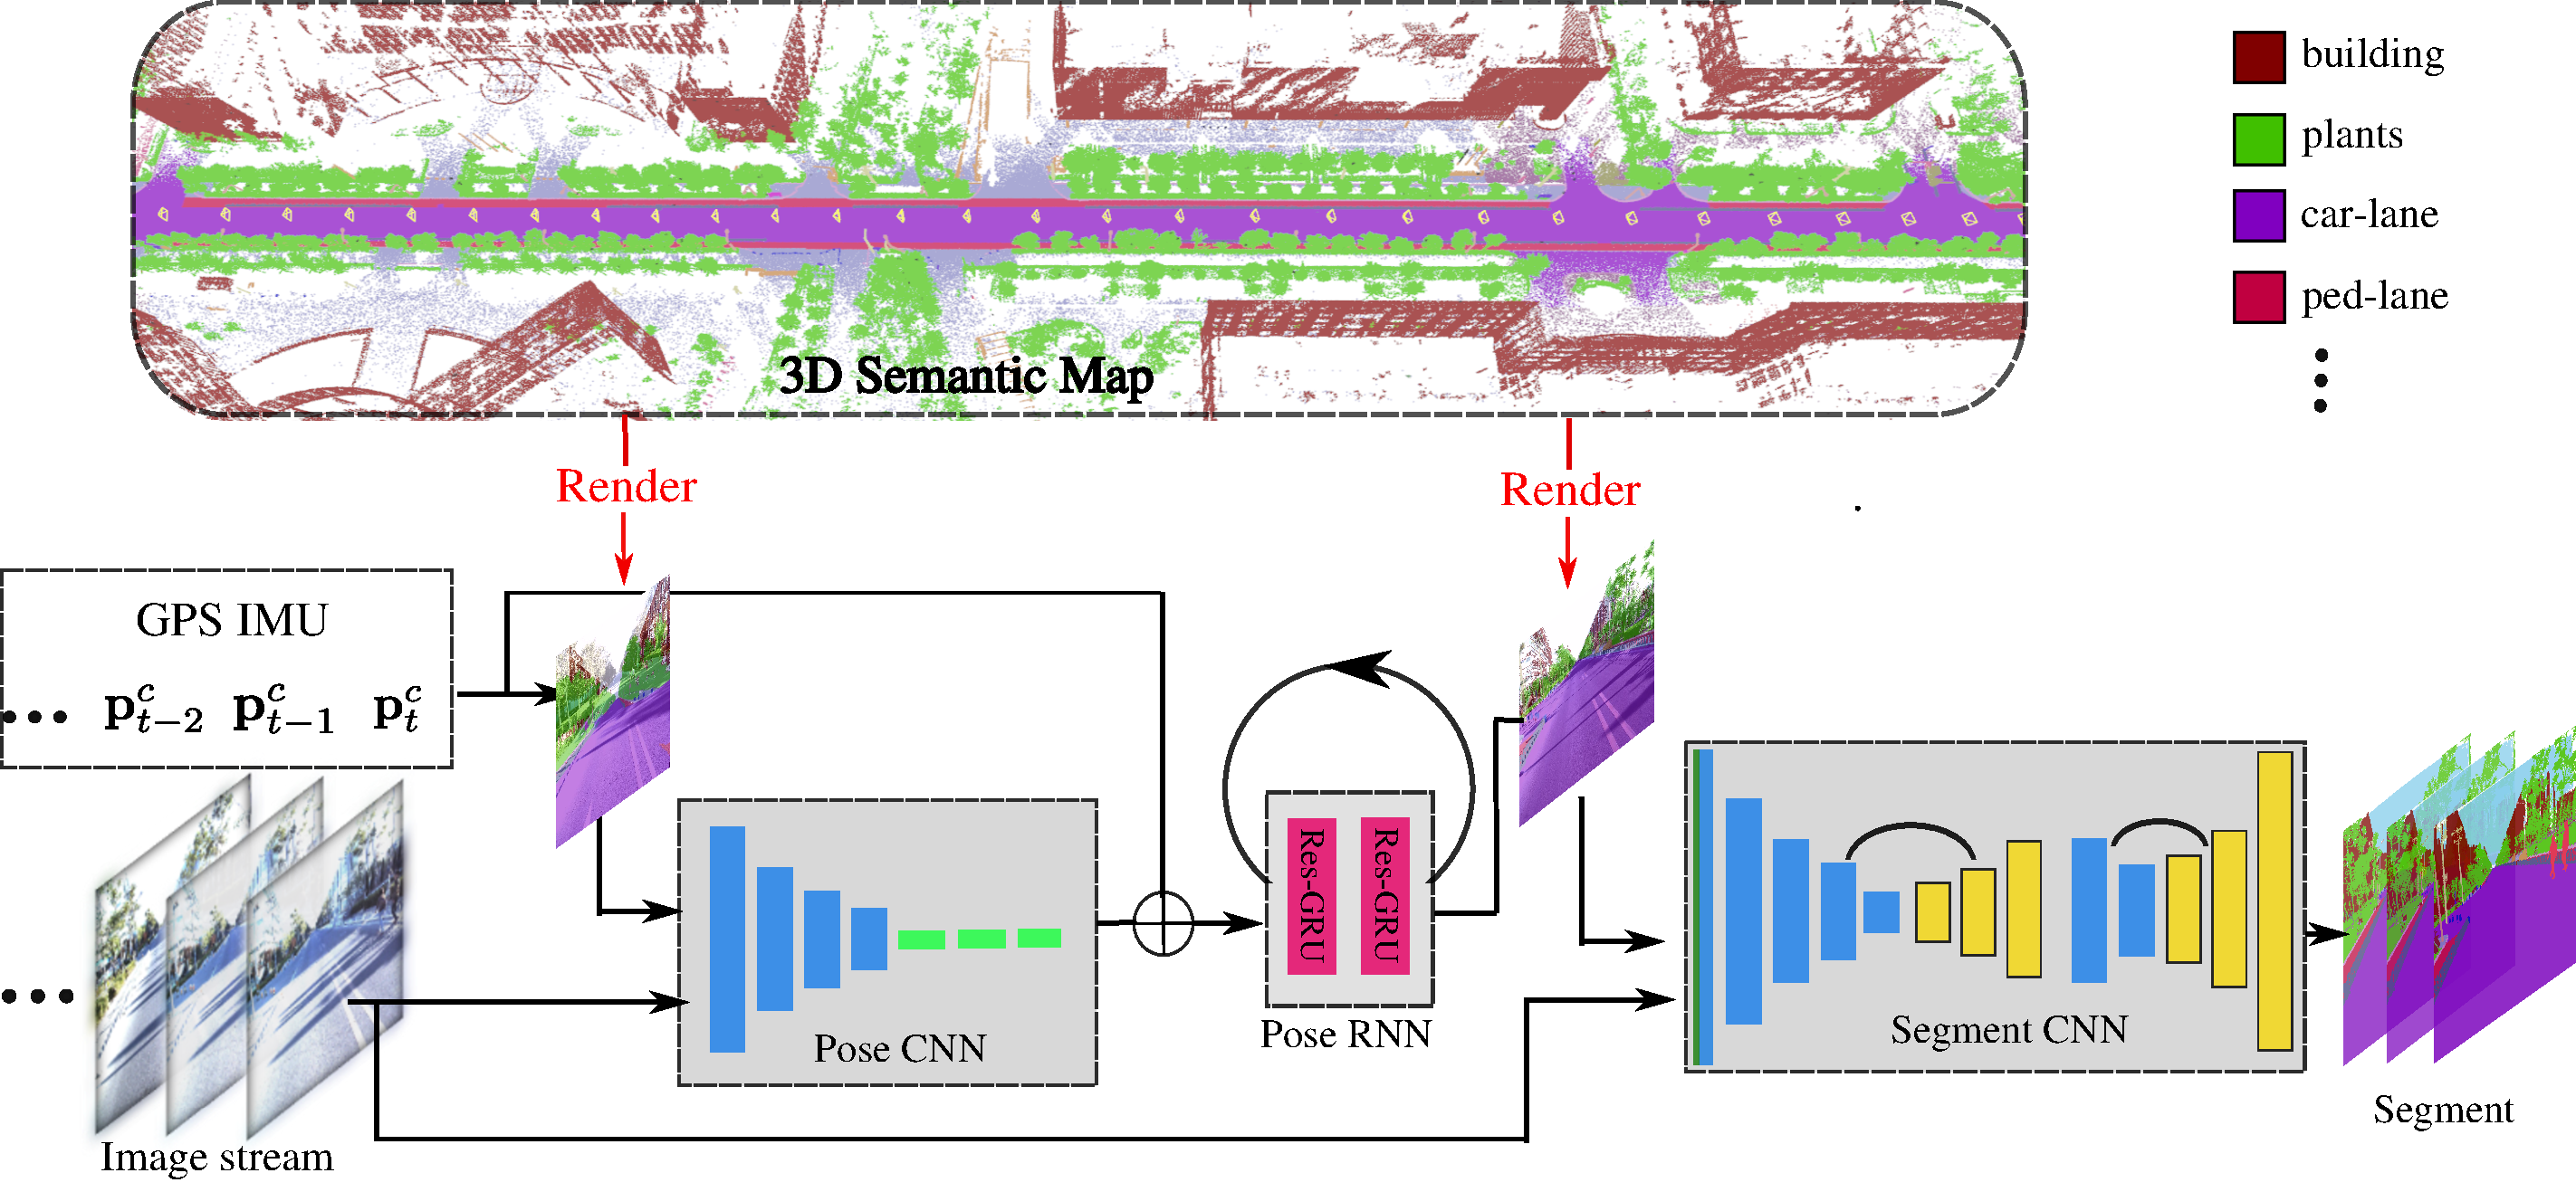
\includegraphics[width=\textwidth]{fig/framework.pdf}
\caption{System overview. The black arrows show the testing process, and red arrows indicate the rendering (projection) operation in training and inference. The yellow symbol shows the trajectory of the cameras.\textcolor{red}{check!} The input of our system contains a sequence of images and corresponding GPS/IMU signals. The outputs are the semantically segmented images, each with its refined poses.}
\label{fig:framework}
\end{figure*}

% existing methods only consider one of the tasks with soly visual signal.
Currently, most existing vision algorithms are trying to solve both tasks solely on visual signals.
For instances, geometric based methods are relying on visual feature matching, \eg~systems of Perspective-n-Points (PnP)~\cite{haralick1994review,kneip2014upnp,campbell2017globally} when a 3D map and an image is provided, or systems of SLAM~\cite{engel2014lsd,mur2015orb,NewcombeLD11} when there is a video. Such systems are relying on local appearance, which could fail when confronted with low-texture environments.

Most recently, deep learning based methods, \eg~for either images~\cite{Kendall_2015_ICCV} or videos~\cite{DBLP:journals/corr/ClarkWMTW17}, have been developed for real-time localization, which show good trade-offs between accuracy and speed.
Nevertheless, those methods are good for environments with rich distinguishable features, such as these in the Cambridge landmarks dataset~\cite{Kendall_2015_ICCV}. They could fail for common street views with very similar appearances or even repetitive structures.
%For example, when driving inside a tree-line street beside, can hardly localize the images without external signals.

For scene parsing, approaches~\cite{ZhaoSQWJ16,ChenPSA17} based on deep fully convolutional network (FCN) with ResNet~\cite{HeZRS15} are the better-performing algorithms for single image input. When the input is video, researchers~\cite{kundu2016feature,zhu2016deep} may incorporate the optical flow between consecutive frames, which not only accelerates the parsing, but also improve temporal consistency. Furthermore, for static background, one may use structure-from-motion (SFM) techniques~\cite{wu2011visualsfm} to jointly parse and reconstruct~\cite{kundu2014joint}. However, these methods can still be fragile in practice.

We aim to solve this camera localization and scene parsing problem from a more practical standpoint. That is, we assume that there will be (a) GPS/IMU signal to provide a rough location estimate; and (b) a semantic 3D map for the static environment. The GPS/IMU signal, even though noisy, serves as the crucial pose prior for our deep-learning based pose estimation system. The semantic 3D map, which could be rendered to a semantic label map for a given pose, not only provides strong priors for scene parsing, but also helps maintain temporal consistency.

%In our scenario, targeting at a more practical setting, we consider the video is online recorded, and a 3D semantic map is pre-built by us. For handling the localization confusion of street views, we propose to fuse signals from motion sensors like global positioning system (GPS) and inertial measurement unit (IMU), which is typically available for current navigation system. Those signals can be noisy but is crucial as a pose priori for our deep learning system.
%For video segmentation, we online render images from the 3D map, which serves as a priori for further segmentation, and helps the consistency along the temporal dimension.
%
In fact, our problem setting is on par with the widely used mobile navigation system, whereas the 2D labeled map is raise up to a 3D semantic map, and the problem of 2D location estimation is changed to 3D camera pose. Promisingly, with the accelerated development of autonomous driving, city-scale 3D semantic maps are being collected and built (such as the Toronto City dataset~\cite{wang2016torontocity}).  In our case, we constructed our own data with high quality 3D semantic map, which is captured by a high-accuracy mobile LIDAR device from $Riegl$\footnote{http://www.rieglusa.com/index.html}.

%lots of city scale 3D map has already collected from companies such as Google Earth~\cite{sheppard2009ethics} and Altizure\footnote{https://www.altizure.com/}, and also semantic labeled ones is also built such as Toronto city~\cite{wang2016torontocity}. In our case, we constructed our own data with high quality 3D semantic map, by adopting a high accuracy mobile LIDAR device from Riegl\footnote{http://www.rieglusa.com/index.html}.

Last but not least, within our deep learning framework, the camera pose and semantics are mutually beneficial, where pose helps establish the correspondences between the 3D semantic map and 2D semantic label map. Conversely, semantics could help refine camera poses. Our unified framework yields better results, in terms of both accuracy and speed, for both tasks than doing them individually. In our experiments, using a single core of Titan Z GPU, our system estimates the pose in 10ms with accuracy under 1 degree, and segments the image $512 \times 608$ in less than 100ms with pixel accuracy around 96$\%$, which demonstrates its efficiency and effectiveness.

% redefine our problem
In summary, the contributions of this paper are:
\begin{itemize}
    \item We propose a deep learning based system for fusing multiple information, \ie~camera images, GPS and IMU, and 3D maps, which helps to improve the robustness and accuracy for camera localization and scene parsing.
    \item Camera pose and scene semantics are handled jointly in both training and testing; they are mutually beneficial.
    \item We construct a dataset from real scenes to fully evaluate our approach. It includes dense 3D semantically labelled point cloud, ground truth camera poses and pixel-level segmentation of every frame, which we will release in order to benefit related research in computer vision.
\end{itemize}

The structure of this paper is organized as follows. We first give a overview of our system in \secref{sub:framework}. In \secref{sec:data_collection}, we first describe how our data is different from the existing outdoor datasets. In addition, we briefly introduce the method how the data is collect and labelled. Then, \secref{sec:localize_and_parsing} presents the framework and detail of our system. The full performance is evaluated quantitatively for both pose estimation and parsing in \secref{sec:experiments}, and \secref{sec:conclusion} concludes the paper and point out future directions. Finally, we will release all our code, models and dataset with the publication of this paper.


\subsection{Framework}
\label{sub:framework}
The framework of our system is illustrated in \figref{fig:framework}. At above, a pre-built 3D semantic map is available. During testing, an online stream of images and corresponding camera poses that is based on GPS/IMU are fed in to the system. Firstly, for each frame, a semantic label map is rendered out based on the input coarse camera pose. Then it is fed to a pose network jointly with the respective image.  The network calculates the relative rotation and translation, and yields a corrected camera pose. To build the temporal correlations, the corrected poses are fed into a RNN which further improves the pose accuracy in the stream.
Last, given the rectified camera pose, a new rendered label map is generated. We feed it together with the image to a segmentation network, which helps to segment a spatially more accurate and temporally more consistent result for the stream of video.
In this system, since our data contains ground truth for both pose and segments, it can be trained with strong supervision at each end of outputs.
